\documentclass[10pt,letterpaper]{article}
\usepackage[margin=.75in]{geometry}
\usepackage{amsmath,amssymb,graphicx,booktabs,xcolor,hyperref,fancyhdr}
\definecolor{navy}{HTML}{18384B}\definecolor{teal}{HTML}{168F9A}\definecolor{pale}{HTML}{EAF4F4}
\hypersetup{colorlinks=true,linkcolor=teal,urlcolor=teal,pdftitle={Waves, dispersion and decay: a visual numerical study},pdfauthor={Dysthe numerical study}}
\pagestyle{fancy}\fancyhf{}\lhead{\small\color{navy}WAVES, DISPERSION AND DECAY}\rhead{\small\color{teal}Numerical study}\cfoot{\color{navy}\thepage}
\setlength{\headheight}{14pt}\setlength{\parindent}{0pt}\setlength{\parskip}{6pt}
\newcommand{\norm}[1]{\left\|#1\right\|}
\newcommand{\eyebrow}[1]{{\color{teal}\normalsize\bfseries #1}\par}
\newcommand{\takeaway}[1]{\par\smallskip\colorbox{pale}{\parbox{.96\linewidth}{\vspace{5pt}\textbf{Read this first.} #1\vspace{5pt}}}\par\smallskip}
\newcommand{\pic}[2]{\begin{center}\includegraphics[width=#1\linewidth]{#2}\end{center}}
\newcommand{\MassError}{$1.11\times10^{-16}$}
\newcommand{\SymmetryError}{$1.76\times10^{-16}$}
\newcommand{\PlaneError}{$2.18\times10^{-15}$}
\newcommand{\ReverseError}{$6.69\times10^{-16}$}
\newcommand{\QuadError}{$3.91\times10^{-9}$}
\newcommand{\PeakPercent}{0.556}
\newcommand{\Runtime}{12.4}
\newcommand{\FinalRows}{$1$ & unshifted & 0.473 & 3.598 & 3.598 & 3.866 \\
$1$ & x shift & 0.438 & 3.891 & 3.598 & 4.140 \\
$1$ & z shift & 0.414 & 4.849 & 4.849 & 3.090 \\
$-1/3$ & unshifted & 0.481 & 3.598 & 3.598 & 3.629 \\
$-1/3$ & x shift & 0.444 & 3.891 & 3.598 & 3.919 \\
$-1/3$ & z shift & 0.303 & 4.849 & 4.849 & 4.872 \\
$0$ & unshifted & 0.467 & 3.598 & 3.598 & 3.598 \\
$0$ & x shift & 0.433 & 3.891 & 3.598 & 3.891 \\
$0$ & z shift & 0.346 & 4.849 & 4.849 & 3.598 \\}
\newcommand{\GridRows}{$32^3$ & $1.89\times10^{-1}$ & $2.05\times10^{-1}$ & $1.68\times10^{-1}$ \\
$64^3$ & $7.75\times10^{-6}$ & $8.24\times10^{-6}$ & $7.38\times10^{-6}$ \\
$96^3$ & $2.13\times10^{-14}$ & $2.15\times10^{-14}$ & $1.90\times10^{-14}$ \\}
\newcommand{\DomainRows}{$1$ & $5.87\times10^{-3}$ & $2.00\times10^{-5}$ & $2.07\times10^{-4}$ \\
$-1/3$ & $3.70\times10^{-2}$ & $1.71\times10^{-5}$ & $1.55\times10^{-5}$ \\
$0$ & $3.95\times10^{-3}$ & $1.49\times10^{-7}$ & $5.58\times10^{-7}$ \\}
\newcommand{\RefinedRows}{Homogeneous & Gaussian & 0.00731 & 1.11\% & 0.18\% \\
Homogeneous & Compact bump & 0.00677 & 0.43\% & 0.03\% \\
Homogeneous & Near degeneracy & 0.00499 & 1.62\% & 0.24\% \\
Homogeneous & Random (33) & 0.00618 & 1.61\% & 0.29\% \\
Inhomogeneous & Gaussian & 0.00468 & 0.01\% & 0.05\% \\
Inhomogeneous & Compact bump & 0.00431 & 0.00\% & 0.54\% \\
Inhomogeneous & Near degeneracy & 0.00344 & 1.36\% & 0.01\% \\
Inhomogeneous & Random (33) & 0.00415 & 0.00\% & 0.04\% \\}
\newcommand{\ObservedResult}{The inhomogeneous Gaussian and random packet ratios begin to flatten: from $t=8$ to $16$ they grow by 3.42\% and 0.78\%, respectively. The near-degeneracy ratios continue to rise more visibly, as do several homogeneous cases. This suggests different transient time scales; it does not establish their eventual behavior.}
\newcommand{\CheckResult}{Across all 24 checked case--time combinations, the largest peak changes are 1.62\% under domain enlargement and 0.94\% under grid refinement. All pass the exploratory 2\% screen.}
\newcommand{\LongRows}{Homogeneous & Gaussian & 0.00917 & 0.00999 & 1.043 \\
Homogeneous & Near degeneracy & 0.00833 & 0.00888 & 1.074 \\
Inhomogeneous & Gaussian & 0.00407 & 0.00372 & 1.293 \\
Inhomogeneous & Near degeneracy & 0.00558 & 0.00586 & 1.096 \\}
\newcommand{\LongDomain}{0.141\%}
\newcommand{\LongQuad}{0.020\%}
\newcommand{\LongEdge}{0.586\%}

\DeclareMathSizes{9}{10}{7}{5}
\DeclareFontShape{OT1}{cmr}{bx}{n}{<->cmbx10}{}
\begin{document}
\thispagestyle{empty}
\eyebrow{A VISUAL NUMERICAL STUDY / SEPTEMBER 2026}
{\color{navy}\Huge Waves, dispersion\\[4pt] and decay}\par
{\Large From individual crests to a three-dimensional decay test}
\pic{1}{visuals/hero.pdf}
\textbf{A wave inside its envelope.} The colored surface is an illustrative carrier
reconstruction on a slice of random seed 33 at $t=4$. The teal mesh follows its
positive envelope. Height means relative amplitude; this is not a third spatial
coordinate or a measured water surface.
\takeaway{The latest computation gives stronger spatial support for four candidate
peaks at $t=256$: all pass a 0.1\% stability screen. It does not yet establish a
sharper decay theorem or a counterexample.}
\textbf{The reading route}\par
\begin{tabular}{@{}ll@{}}
\textcolor{teal}{02--03} & Understand the envelope and the fluid analogy.\\
\textcolor{teal}{04--06} & Explore random 3D packets and the weighted diagnostic.\\
\textcolor{teal}{07--10} & Read the long-time results and the broader data collection.\\
\textcolor{teal}{11--18} & Inspect equations, numerical checks, and reproduction details.\\
\textcolor{teal}{19--22} & Explore the new research-motivated experiments.
\end{tabular}
\vfill
{\small Scope: linear optical dispersion and canonical weighted propagators associated
with the supplied Dysthe manuscript. The full nonlinear water-wave system is not simulated.}
\newpage
\eyebrow{01 / READING A WAVE}
\section*{The magnitude is the height of an envelope}
The complex envelope carries amplitude and phase. Its magnitude tells us how
large the local oscillations can be; it is not velocity. A carrier supplies the
rapid crests and troughs inside that slowly varying outline.
\pic{1}{figures/envelope_explanation.pdf}
\takeaway{The oscillating curve is the wave. The upper and lower outlines are
$+|E|$ and $-|E|$. A magnitude plot shows that outline, without drawing each crest.}
The schematic reconstruction is
\[u_{\rm carrier}=\operatorname{Re}\{E\,e^{i\phi_{\rm carrier}}\}.\]
Phase matters: two envelopes with the same magnitude can produce different crest
positions and different interference. The figures on page 5 retain the simulated
complex phase and add a visible carrier for illustration.

Optical intensity is proportional to $|E|^2$. A peak magnitude of $0.47$ corresponds
to about $0.22$ of the initial peak intensity when the initial amplitude is one.
Spreading can lower this peak while preserving the integral of $|E|^2$.

\textbf{Units and normalization.} Computations are dimensionless. The early optical
Gaussian examples start at peak one. Canonical decay inputs instead have $L^1=1$.
Their small numerical amplitudes reflect this different normalization and should
not be compared directly with the optical peaks.
\newpage
\eyebrow{02 / A FLUID ANALOGY}
\section*{What a packet looks like on water}
A group contains several crests: they grow toward its center and fade near its
edges. The envelope is an outline of their amplitude, not another material surface.
\pic{.94}{figures/water_packet.pdf}
For small-amplitude deep-water gravity waves, $c_g=c_p/2$: individual crests
move through the group. The dots in the lower panels track phase and group position,
not water parcels. This illustration uses wavelength 4 m and amplitude 0.08 m,
with vertical exaggeration. It omits spreading, nonlinear corrections and breaking.
\takeaway{A surface plot has two horizontal coordinates and elevation. Our 3D
field has three independent coordinates: its amplitude must be shown by color,
slices, or level surfaces, as on the next page.}
{Fluid interpretation: R. Salmon, \href{https://www-pord.ucsd.edu/rsalmon/111.textbook.pdf}{\emph{Introduction to Ocean Waves}}, Chapter 2, pp. 25--26. This is an explanatory analogy, not output from a fluid solver.}
\newpage
\eyebrow{03 / THREE REPRODUCIBLE RANDOM CASES}
\section*{A volume can stretch, split and move}
\pic{.68}{visuals/random_volumes.pdf}
{\small Each surface encloses $|S(t)f|\geq0.3\max|S(t)f|$ on the sampled volume.
All axes are spatial, with the same viewing window. Thresholds follow each
snapshot's own peak: compare shape here, and use the printed peaks to compare
amplitude. These are three fixed seeds, not a statistical sample.}
\newpage
\eyebrow{04 / LOOKING INSIDE THOSE PACKETS}
\section*{The individual oscillations remain visible}
\pic{1}{visuals/random_carriers.pdf}
The dark curves show $\operatorname{Re}\{S(t)f(x,0,0)e^{3ix}\}$; colored outlines
show $\pm|S(t)f(x,0,0)|$. Each row uses its initial slice peak as a fixed divisor,
so changes in amplitude remain visible between its two panels.
\takeaway{An envelope does not erase individual waves. It describes their local
amplitude and phase; an extra carrier reconstructs oscillations. The carrier
wavenumber 3 here is chosen for readability, not inferred from physical data.}
{\small Gallery computation: homogeneous canonical symbol, $128^3$ periodic grid,
length 96, spacing 0.75, seeds 11/22/33. Each input is a Gaussian window times 12
random Fourier modes, normalized to discrete $L^1=1$. These are qualitative
short-time views; the $t=256$ spatial audit does not apply to them.}
\newpage
\eyebrow{05 / FROM PICTURES TO AN INEQUALITY}
\section*{Which quantity must decay?}
A shrinking envelope peak is suggestive, but the paper bounds a different field:
a fractional Fourier multiplier is applied before taking its maximum.
\[W(t)=|D_x+\beta|^{1/2}S(t)f,\qquad
\widehat W=|k_x+\beta|^{1/2}e^{itw}\widehat f.\]
\pic{1}{visuals/weighted_comparison.pdf}
\textbf{Same input, different quantity.} Seed 33 at $t=4$, on the $y=0$ plane.
Each panel has its own amplitude scale. The right panel is the field used in the
inequality; it is not surface elevation or velocity.
\[\boxed{R(t;f)=\frac{t^{7/6}\|W(t)\|_\infty}{\|f\|_1}\leq C}\]
For $\alpha=1/2$, the predicted comparison rate is $t^{-7/6}$. The constant must
be independent of input and time at fixed equation parameters.
\begin{center}\begin{tabular}{ll}\toprule
If the ratio $R(t)$ is\ldots & The weighted peak behaves\ldots\\\midrule
Flat & Like $t^{-7/6}$ over that interval.\\
Falling & Faster than $t^{-7/6}$ over that interval.\\
Rising & Slower than $t^{-7/6}$ over that interval.\\\bottomrule
\end{tabular}\end{center}
\takeaway{The claim is boundedness, not monotonicity. A rising finite curve can
still approach a finite constant. Many inputs make the experiment more searching;
they do not by themselves turn it into a uniform theorem.}
\newpage
\eyebrow{06 / THE LONG-TIME RESULT}
\section*{Following four cases through $t=256$}
\pic{1}{../results/long_time/decay_256.pdf}
The inhomogeneous Gaussian ratio falls at late times; the other three rise over
the last doubling. Those are finite-time trends, not asymptotic conclusions.
\begin{center}\small\begin{tabular}{llrrr}\toprule
Equation & Input & $R(128)$ & $R(256)$ & Local exponent\\\midrule
\LongRows\bottomrule\end{tabular}\end{center}
The exponent is $-\log[M(256)/M(128)]/\log2$, where $M=\|W\|_\infty$.
Compare it with $7/6\simeq1.167$; it describes one time doubling only.
These curves and entries retain the long-time batch values. The subsequent audit
refines the four endpoint ratios in the technical table at the end of this report.
\takeaway{We now have a longer observation window. The strongest result is the
improved reliability of its four endpoint peaks, shown next. No counterexample
or stronger uniform exponent has been established.}
\newpage
\eyebrow{07 / CAN WE TRUST THE SPATIAL COMPUTATION?}
\section*{Enlarge the search, then compare again}
At fixed $t=256$, we increased the longitudinal period from 32,768 to 65,536 and
then 131,072. Separately, the radial search grew from 2,048 to 4,096. The broad
search retained $\Delta x=0.25$ and $\Delta r=2$, followed by local peak optimization.
\pic{1}{visuals/reliability.pdf}
\takeaway{All four cases pass the 0.1\% numerical screen. The largest final
change in refined peak magnitude is 0.00459\%; the largest location drift is
0.00079 spatial units.}
An independent non-periodic integral agrees within 0.0026\% at the candidate peaks.
Extending the radial search found no larger sampled maximum. These checks support
stability under the tested changes, rather than supplying a rigorous error bound.

\textbf{Why length matters.} The inhomogeneous near-degeneracy peak is near
$x=-841$ at $t=256$. It lies far outside the length-288 box used for the earlier
experiments. A long-time curve on that old box could confuse periodic recirculation
with whole-space behavior.

\textbf{What remains unresolved.} A finite search and local refinement can miss a
narrow or distant maximum. This audit covers four Gaussian-based cases at one time
and one derivative weight. It does not transfer automatically to random inputs.
\newpage
\eyebrow{08 / BEYOND A SINGLE GAUSSIAN}
\section*{Eleven families make the test more varied}
\pic{.98}{../results/decay_dataset/families_clear.pdf}
{\small Original short-time survey: two equation regimes per panel, $\alpha=1/2$,
length-96 box. These curves remain exploratory finite-box measurements. Recipes
include compact, anisotropic, chirped, tapered algebraic and random inputs.
The three random seeds shown earlier belong to this collection. No measured
fluid dataset has been imported.}
\newpage
\eyebrow{09 / A MORE CAREFUL INTERMEDIATE WINDOW}
\section*{Four families checked through $t=16$}
\pic{1}{../results/decay_dataset/refined_clear.pdf}
Curves use a length-288 cube at spacing 1. Dots identify the checked times
$t=4,8,16$ passing the exploratory 2\% peak-change screen in both domain and grid
comparisons; intermediate times were not independently checked.
\takeaway{Across 24 checked case--time combinations, the largest domain peak
change is 1.62\% and the largest grid peak change is 0.94\%. This supports the
intermediate-time comparisons, with weaker tolerances than the four-case endpoint audit.}
\textbf{Next scientific step.} Extend the reliable time window for more recipes,
keeping input normalization fixed and testing spatial stability at each new stage.
A candidate contradiction needs sustained growth that survives those checks;
strengthening a uniform theorem needs an argument covering its full input class.

\textbf{Technical record follows.} The remaining pages retain the equations,
optical baseline results, detailed refinement tables and reproducible algorithms.
The optical plots use an unweighted field and a different normalization from the
canonical ratio experiments; they explain dispersion but are not direct bound tests.
\newpage
\eyebrow{TECHNICAL RECORD / OPTICAL BASELINE}
\section*{1. Equation and numerical model}
We solve
\begin{equation}
 iE_t+(1-i\varepsilon_1\partial_z)\Delta_\perp E-E_{zz}
       -i\varepsilon_2 E_{zzz}=0,
 \qquad \Delta_\perp=\partial_x^2+\partial_y^2.
 \label{eq:pde}
\end{equation}
With $\widehat E(\mathbf k)=\int E(\mathbf x)e^{-i\mathbf k\cdot\mathbf x}\,d\mathbf x$,
\begin{equation}
 \widehat E(\mathbf k,t)=e^{-it\omega(\mathbf k)}\widehat E_0(\mathbf k),\qquad
 \omega=(1+\varepsilon_1 k_z)(k_x^2+k_y^2)-k_z^2+\varepsilon_2k_z^3.
 \label{eq:prop}
\end{equation}
This matches the paper's symbol (6.6). Its equation (1.32) prints the opposite sign
on the mixed third derivative. We follow (1.27) and (6.6) consistently; this choice
must be retained when comparing with another implementation.

An FFT computes the initial coefficients once. For each requested $t$, we multiply
by the phase in \eqref{eq:prop} and perform an inverse FFT. Evolution of the retained
modes is exact up to floating-point arithmetic. There is no time-marching truncation
error; spatial sampling, finite-box effects, and sampling the peak remain relevant.
At a fixed total grid size $N$, $M$ snapshots cost $O(MN\log N)$.

\begin{center}
\begin{tabular}{ll}\toprule
Setting & Value \\\midrule
Computational box & $[-48,48)^3$, periodic \\
Production grid & $96^3$ points; $\Delta x=\Delta y=\Delta z=1$ \\
Arithmetic & Torch CPU, complex128, four threads \\
Evolution times & 25 snapshots, $t=0,0.25,\ldots,6$ \\
Parameters & $\varepsilon_1=1$; $\varepsilon_2\in\{1,-1/3,0\}$ \\
Initial Gaussian & $E_0=e^{-(x^2+y^2+z^2)/18}e^{i\mathbf q\cdot\mathbf x}$ \\
Frequency shifts & $\mathbf q=0$, $(\pi/6,0,0)$, $(0,0,\pi/6)$ \\\bottomrule
\end{tabular}
\end{center}
The shift is eight Fourier bins on the production box. All three initial magnitudes
are identical, with peak one. Positive $\varepsilon_2$ and $-\varepsilon_1/3$ connect
to the parameter cases in Theorem 5.1; the zero case is included as a linear comparison,
without extending that nonlinear theorem to it. All quantities are dimensionless.

\newpage
\section*{2. Peak evolution and parameter dependence}
The peak curves below are spatial grid maxima, not amplitudes at a fixed point.
All three parameter families spread over the observation window. The response to
a $z$-shift depends strongly on $\varepsilon_2$, even though the initial magnitudes
and norms are unchanged.
\begin{center}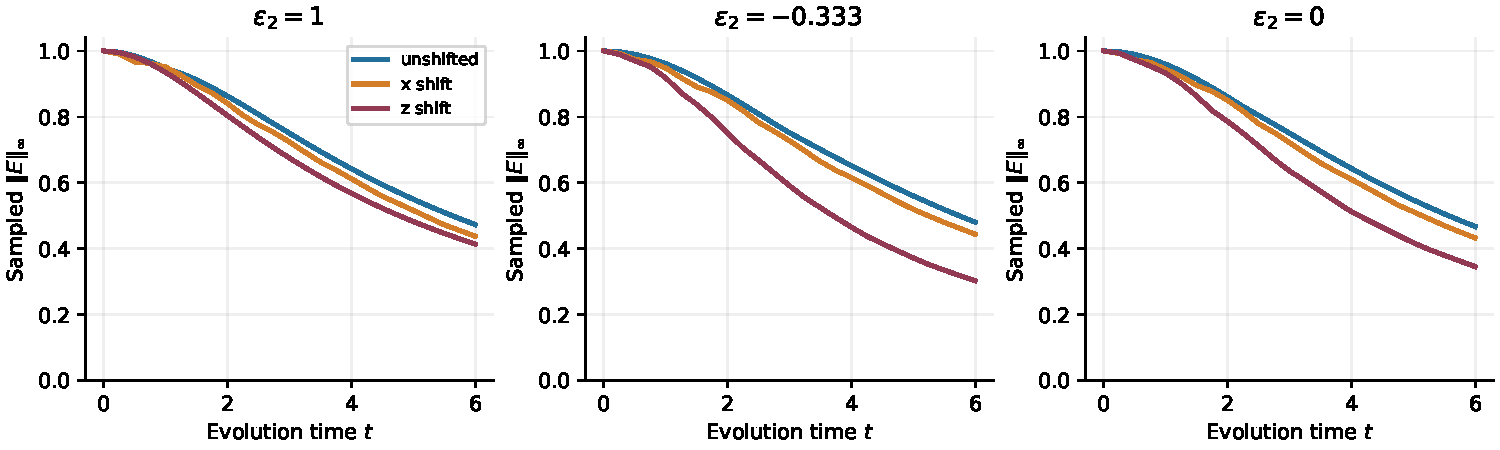
\includegraphics[width=\linewidth]{figures/peak_decay.pdf}\end{center}
\textbf{Figure 3.} Sampled $L^\infty$ histories. Lines join directly evaluated
snapshots; they do not represent a numerical time integrator.

\begin{center}
\begin{tabular}{llrrrr}\toprule
$\varepsilon_2$ & Initial spectrum & Peak at $t=6$ & $s_x$ & $s_y$ & $s_z$ \\\midrule
\FinalRows
\bottomrule\end{tabular}
\end{center}
Here $s_j$ is the standard deviation of coordinate $j$ under the normalized intensity
$|E|^2/\int|E|^2$. Initially $s_x=s_y=s_z=3/\sqrt2\simeq2.121$.
Widths describe the packet as a whole and remain meaningful when its maximum moves.

For $\varepsilon_2=1$, the final peaks are approximately $0.473$ (unshifted),
$0.438$ ($x$-shift), and $0.414$ ($z$-shift). For $\varepsilon_2=-1/3$, the
$z$-shifted peak is approximately $0.303$. The $z$-shift therefore need not have
the same effect across dispersion parameters.

\textbf{What these curves establish.} They demonstrate finite-time spreading and
directional sensitivity for these initial data. They do not establish an asymptotic
decay exponent, monotone decay for arbitrary data, or a universal decay constant.
The reported $L^2$ norm is constant to relative error \MassError; this is
dispersion without imposed damping.

\newpage
\section*{3. Spatial solutions}
\begin{center}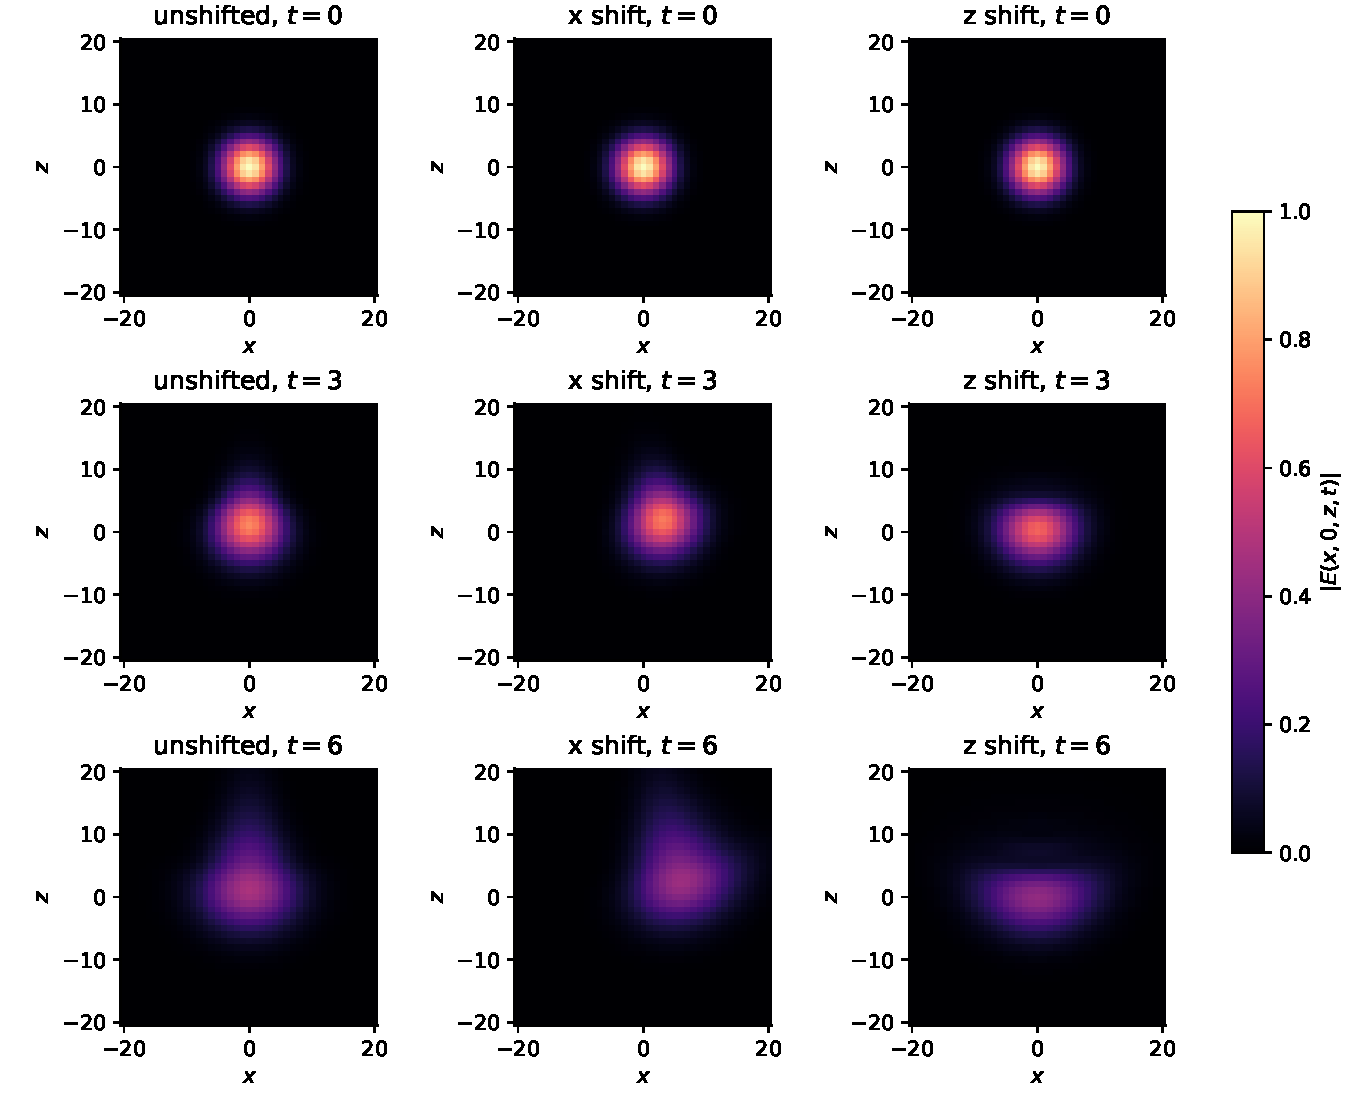
\includegraphics[width=.97\linewidth]{figures/slices.pdf}\end{center}
\textbf{Figure 4.} Magnitude on the $y=0$ plane for $\varepsilon_2=1$. Columns
compare unshifted, $x$-shifted, and $z$-shifted initial spectra. Rows show
$t=0,3,6$. Every panel uses the same color range, making the loss of peak
amplitude visible. The displayed window is $[-20,20]^2$ within the larger
computational box; the color plots are slices of genuine three-coordinate solutions.

Modulation changes propagation as well as deformation. A slice alone can miss
an off-plane maximum, which is why Figure 3 and the table use the full volume.
Full complex fields at $t=6$ are supplied in the accompanying snapshot archive.

\newpage
\section*{4. Directional spreading and generic initial data}
\begin{center}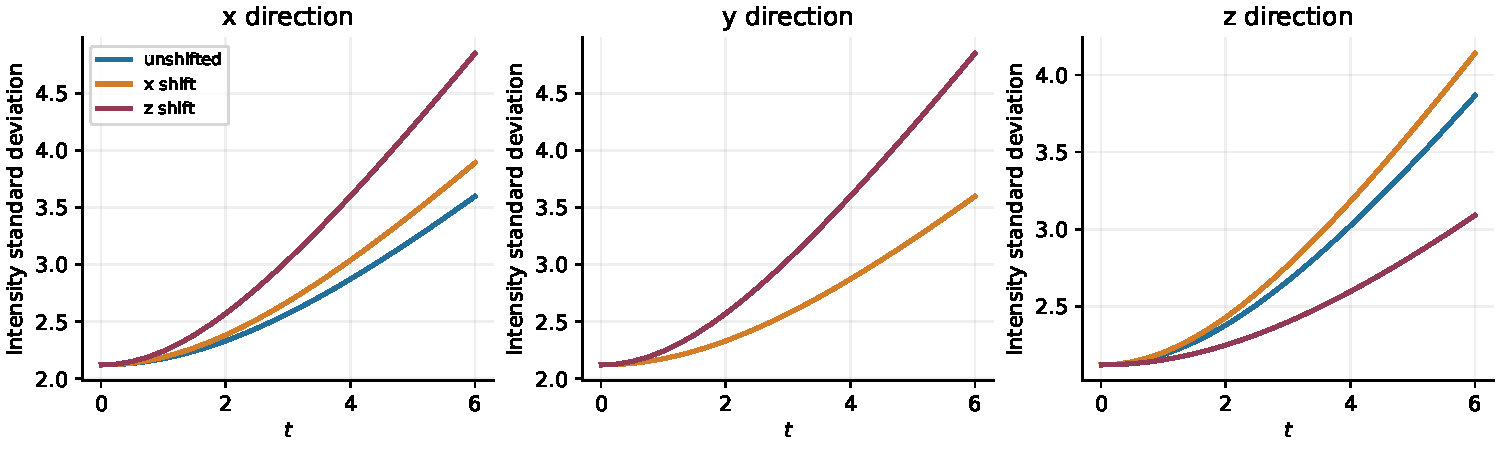
\includegraphics[width=\linewidth]{figures/widths.pdf}\end{center}
\textbf{Figure 5.} Intensity widths for $\varepsilon_2=1$. An $x$-shift breaks
the equality of the transverse widths; a $z$-shift changes both transverse widths
together. Exchanging $x$ and $y$ in the shifted experiment agrees to maximum
absolute field error \SymmetryError.

This behavior is consistent with the group velocity of \eqref{eq:prop}:
\[
 \nabla_{\mathbf k}\omega=
 \bigl(2(1+\varepsilon_1k_z)k_x,\;
       2(1+\varepsilon_1k_z)k_y,\;
       \varepsilon_1(k_x^2+k_y^2)-2k_z+3\varepsilon_2k_z^2\bigr).
\]
Changing $k_z$ changes the transverse dispersion factor itself. Changing $k_x$
also affects longitudinal transport through the $k_x^2$ term. The axes are coupled.

\begin{center}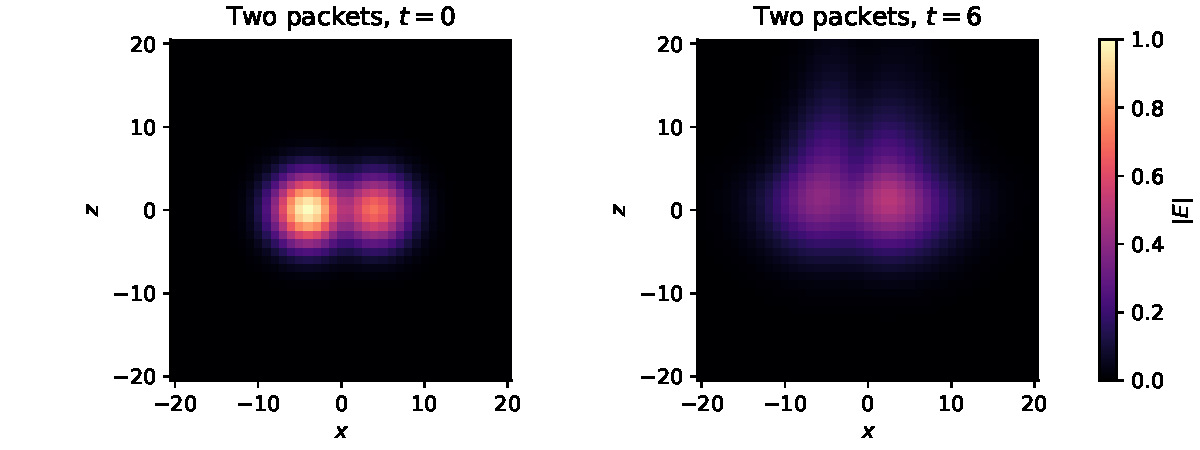
\includegraphics[width=.85\linewidth]{figures/generic.pdf}\end{center}
\textbf{Figure 6.} A non-Gaussian initial profile, propagated with the same solver:
\[
 E_0=e^{-((x+4)^2+y^2+z^2)/18}
       +0.7i\,e^{-((x-4)^2+y^2+z^2)/18},\qquad \varepsilon_2=1.
\]
This example demonstrates that the solver accepts a sampled complex field without
requiring a Gaussian formula. Its separate convergence study is not included here.

\newpage
\setlength{\parskip}{4pt}
\section*{5. Verification and interpretation limits}
\textbf{Algebraic checks.} A periodic plane wave with wavevector $(1,2,-1)$ at
$\varepsilon_1=\varepsilon_2=1$ has $\omega=-2$, hence exact multiplier $e^{2it}$.
The solver agrees at $t=0.73$ to \PlaneError\ in maximum error. Forward/backward
propagation of the $z$-shifted packet gives relative $L^2$ error \ReverseError.
These checks complement conservation, which alone cannot detect a wrong phase sign.

\textbf{Grid refinement.} The table compares the $z$-shifted field at $t=6$ against
a $192^3$ computation on the same length-96 box. The reference is restricted to
the coarse nodes before measuring relative discrete $L^2$ error.
\begin{center}\begin{tabular}{rrrr}\toprule
Grid & $\varepsilon_2=1$ & $\varepsilon_2=-1/3$ & $\varepsilon_2=0$ \\\midrule
\GridRows
\bottomrule\end{tabular}\end{center}
This demonstrates convergence of sampled fields on a fixed periodic box. It does
not imply that a grid maximum equals the continuum supremum. Across all nine final
Gaussian fields, doubling the resolution changes the sampled peak by at most
\PeakPercent\ percent. Figure 3 retains the production-grid maxima.

\textbf{Domain enlargement.} At spacing $0.5$, length-48 and length-72 boxes are
compared to length 96 on the common cube $[-24,24)^3$, using the $z$-shifted field.
A separate check compares each production field to a length-144 box at spacing 1,
restricted to the entire original box. The last column is the worst of all three shifts.
\begin{center}\begin{tabular}{rrrr}\toprule
$\varepsilon_2$ & $L=48$ vs. 96 & $L=72$ vs. 96 & $L=96$ vs. 144 \\\midrule
\DomainRows
\bottomrule\end{tabular}\end{center}
Values are relative discrete $L^2$ differences on the stated comparison regions.
The agreement improves on enlarging the box, but it is evidence on $0\le t\le6$,
not permission to extrapolate indefinitely on a periodic domain.

\textbf{Independent whole-space check.} For the Gaussian, the transverse Fourier
integrals can be evaluated analytically, leaving a one-dimensional adaptive integral
in $k_z$. At $t=6$, we compare the origin, $(3,-2,5)$, and the production peak node
for each of the nine cases. The largest absolute complex-field discrepancy is
\QuadError. Quadrature uses $k_z\in[-5,5]$ with absolute and relative tolerance
$10^{-12}$; Gaussian tails outside this interval are negligible at this precision.
This checks 27 points, not the entire continuum field.

\textbf{Relation to the paper.} Propositions 6.2--6.3 bound a fractional-derivative-weighted
solution in transformed coordinates for $0<\alpha<1$. They do not directly assert
the plotted unweighted peak follows $t^{-(3+\alpha)/3}$. No exponent is fitted here,
and no theorem constant is inferred. The weighted experiments earlier in this combined report address that separate diagnostic.

\textbf{Reproduction.} From the project folder, run the following commands:
\begin{quote}\small\ttfamily
python3 numerical\_solutions.py\\
python3 report/make\_tables.py
\end{quote}
Compile \texttt{unified\_report.tex} from \texttt{report/}. Dependencies are NumPy, SciPy, Matplotlib, and Torch.
The supplied CSV contains all 225 Gaussian norm records; JSON contains checks and
configuration; the NPZ contains nine final Gaussian fields and the two-packet field.
The recorded computation and figure-generation time was \Runtime\ seconds on this
host; this is one CPU run, not a hardware benchmark or a GPU measurement.

\textbf{Source.} R. Mosincat, D. Pilod, and J.-C. Saut,
\emph{On Third Order Nonlinear Schr\"odinger Equations}, supplied manuscript
\texttt{Dysthe3D-2.pdf}, pp. 9--10 and 18--23. No publication status is assumed.
\newpage
\eyebrow{TECHNICAL RECORD / CANONICAL PROPAGATOR}
\section*{Weighted equation and intermediate checks}
We use $S(t)f=\mathcal F^{-1}(e^{itw}\widehat f)$ with
\[w=k_x^3+3s k_x(k_y^2+k_z^2)+3\beta(k_y^2+k_z^2),\]
where $(s,\beta)=(-1,0)$ or $(1,1)$. This follows the proofs of Propositions
6.2--6.3; the signs printed in (6.1) are inconsistent. The weighted multiplier is
$|k_x+\beta|^{1/2}$. These are canonical coordinates, not a numerical conversion
of the optical baseline above.

We extend four families in both regimes to $t=16$, four times the first batch's
maximum time. Gaussian is the reference, the compact bump has a broader spectrum,
the near-degeneracy packet targets the multiplier's cusp, and seed 33 represents
the random collection. This is a targeted follow-up, not an exhaustive data search.

Domain checks compare lengths 96, 192, and 288 at spacing 1. A separate length-192
grid with spacing $2/3$ checks resolution. Every comparison uses the same continuum
recipe, normalized using its own grid quadrature. The table gives results at $t=16$;
machine-readable files also include $t=4,8$ and complex-field errors on a common cube.

\begin{center}\small
\begin{tabular}{llrrr}\toprule
Equation & Input & $R(16)$ & Domain peak change & Grid peak change\\\midrule
\RefinedRows
\bottomrule\end{tabular}
\end{center}
Domain peak change compares lengths 192 and 288; grid peak change compares
spacings 1 and $2/3$ at length 192. Peak comparisons use each grid's full sampled
maximum, not a fixed spatial point. The plotted length-288 field is not itself
also refined to spacing $2/3$, so the checks do not establish joint convergence.

\textbf{Observed behavior.} \ObservedResult

\textbf{Numerical qualification.} \CheckResult
The fractional multiplier can produce long spatial tails, and errors can vary
nonmonotonically with box size near its cusp. A field's relative $L^2$ difference
and its maximum-amplitude difference are distinct: this follow-up prioritizes the
maximum because it appears in the inequality, while retaining both diagnostics.

\textbf{Inference.} These experiments do not establish a faster universal decay
rate, a theorem constant, or a counterexample. A convincing candidate violation
would require a controlled sequence of times or normalized inputs with increasing
ratios that survives numerical refinement. A short transient slope is insufficient.
Cases that fail the peak checks should be refined before being interpreted as
evidence about the whole-space bound.

\textbf{Data and reproducibility.} Run \texttt{python3 decay\_dataset.py}, then
\texttt{python3 refine\_decay.py}. Results are in
\texttt{results/decay\_dataset/}: \texttt{refined\_decay.csv},
\texttt{refinement\_checks.json}, \texttt{REFINEMENT.md}, and the plotted figures.
The first batch's inputs remain available as complex-valued NPZ arrays.
These are artificial inputs. CDIP buoy observations have been identified as a
possible source, but are not imported or presented as three-dimensional measurements.

\textbf{Source.} R. Mosincat, D. Pilod, and J.-C. Saut,
\emph{On Third Order Nonlinear Schr\"odinger Equations}, supplied manuscript
\texttt{Dysthe3D-2.pdf}, Section 6. This supplement follows the stated estimates
as research targets, without claiming to resolve the manuscript's proof details.

\textbf{Visual gallery reproduction.} Run \texttt{python3 report/make\_visual\_gallery.py}.
The script records seeds, grid, normalization, peak values and $L^2$ norms in
\texttt{report/visuals/gallery\_manifest.json}. Rebuild this combined source with
\texttt{python3 report/build\_unified.py}, then compile \texttt{report/unified\_report.tex}.
\newpage
\section*{How the long-time calculation is checked}
Let $r=\sqrt{y^2+z^2}$ and use the exactly $L^1$-normalized initial profile
\[
 f(x,r)=\frac{\exp[-x^2/(2\sigma_x^2)-r^2/(2\sigma_y^2)]e^{iqx}}
 {(2\pi)^{3/2}\sigma_x\sigma_y^2}.
\]
The Gaussian has $(\sigma_x,\sigma_y,q)=(3,3,0)$; the near-degeneracy packet
has $(6,3,-\beta)$. Analytically integrating both transverse Fourier variables
reduces the weighted field to
\[
 W(x,r,t)=\frac1{4\pi^2}\int_{\mathbb R}
 \frac{|k+\beta|^{1/2}}{d(k,t)}
 \exp\!\left[-\frac{\sigma_x^2(k-q)^2}{2}+i(tk^3+kx)
             -\frac{r^2}{2d(k,t)}\right]dk,
 \qquad d(k,t)=\sigma_y^2-6it(sk+\beta).
\]
This is the same three-coordinate linear solution for these inputs. Only the
evaluation method changes. The transverse directions are treated on the whole
space; a longitudinal FFT quadrature evaluates many $x$ locations efficiently.
Radial symmetry reduces the spatial peak search to $(x,r)$.

\begin{center}\begin{tabular}{lrrrr}\toprule
Check & $x$ period & $\Delta x$ & Max. $r$ & $\Delta r$\\\midrule
Base & 4096 & 0.5 & 512 & 4\\
Expanded & 8192 & 0.5 & 1024 & 4\\
Refined & 8192 & 0.25 & 1024 & 2\\
Extra expansion at $t=256$ & 32768 & 0.25 & 2048 & 2\\\bottomrule
\end{tabular}\end{center}
The full $(x,r)$ search is followed by local optimization of the peak. At $256$,
the extra expansion changes the sampled peak by at most \LongDomain. An independent
adaptive quadrature of the integral above agrees with the complex field at each
final candidate peak to within \LongQuad\ relative error. The largest sampled
search-boundary amplitude is \LongEdge\ of its case's peak. These checks are
numerical evidence, not a certification that no larger unsampled peak exists.

\textbf{Why the previous box was inadequate.} At $t=256$, the inhomogeneous
near-degeneracy maximum lies around $x=-841$. It would be outside even the
length-288 box used for the earlier $t\le16$ runs. Extending time without changing
the spatial computation would therefore be unreliable.

\textbf{Remaining limits.} The Gaussian-specific reduction cannot be applied
unchanged to arbitrary measured fields or every artificial recipe. The adaptive
quadrature checks selected peak locations; the global search remains finite and
sampled. The two-dimensional radial search, local optimizer status, boundary ratios,
and domain/resolution comparisons are all recorded to make these limits reviewable.

\textbf{Reproduce.} Run \texttt{python3 long\_time\_decay.py}, followed by
\texttt{python3 report/make\_long\_time\_tables.py}. Results and the graph are under
\texttt{results/long\_time/}; compile \texttt{report/unified\_report.tex} for this
combined numerical study. Source: the same manuscript, canonical symbols (6.2) and
weighted estimates in Propositions 6.2--6.3.

\newpage
\newcommand{\SpatialRows}{Homogeneous & Gaussian & 0.0130\% & 0.0000\% & 0.0046\% & 0.0025\% \\
Homogeneous & Near degeneracy & 0.0020\% & 0.0000\% & 0.0007\% & 0.0003\% \\
Inhomogeneous & Gaussian & 0.0001\% & 0.0000\% & 0.0000\% & 0.0000\% \\
Inhomogeneous & Near degeneracy & 0.0033\% & 0.0000\% & 0.0026\% & 0.0004\% \\}
\newcommand{\SpatialLocations}{Homogeneous & Gaussian & 0.0099887 & -20.7469 & 0.0000 & 0.00000 \\
Homogeneous & Near degeneracy & 0.0088803 & 7.7961 & 6.5381 & 0.00079 \\
Inhomogeneous & Gaussian & 0.0037238 & -8.9154 & 0.0000 & 0.00002 \\
Inhomogeneous & Near degeneracy & 0.0058621 & -841.2464 & 0.0000 & 0.00021 \\}
\newcommand{\SpatialLocationDrift}{0.00079}
\newcommand{\SpatialPeakDrift}{0.00459\%}
\newcommand{\SpatialQuadTighten}{$3.67\times10^{-12}\%$}
\newcommand{\SpatialBoundary}{0.00516\%}
\newcommand{\SpatialPassed}{4}

\section*{Stronger spatial reliability at $t=256$}
\textbf{Purpose.} Hold time, input, and $\alpha=1/2$ fixed, and vary the spatial
computation. This audit separates longitudinal enlargement from transverse
enlargement. It tests whether the four reported candidate maxima stabilize to
an exploratory relative tolerance of $0.1\%$.

The longitudinal period increases from 32,768 to 65,536 while the radial limit
stays at 2,048. We then search the additional annulus out to radius 4,096.
Finally, we double the longitudinal period again to 131,072, retaining the
larger radial limit. Every broad scan keeps $\Delta x=0.25$ and $\Delta r=2$.
The baseline is the saved final scan from the preceding experiment.

\begin{center}\small
\begin{tabular}{llrrrr}\toprule
Equation & Input & First $L$ change & Radius change & Second $L$ change & Integral check\\\midrule
\SpatialRows
\bottomrule\end{tabular}\end{center}
The three domain columns compare sampled peak magnitudes before and after the
stated expansion. The integral check compares the final Fourier-quadrature field
to an independently evaluated non-periodic integral at the refined candidate peak.
Percentages use the newer or independent result as the denominator. Values are rounded.

\textbf{Result.} \SpatialPassed\ of four cases pass the $0.1\%$ peak screen.
This includes the two longitudinal expansions, the transverse expansion, the
final locally optimized peak drift, and the independent integral check.
The largest change in locally optimized peak magnitude between the final two
periods is \SpatialPeakDrift.

\begin{center}\small
\begin{tabular}{llrrrr}\toprule
Equation & Input & Refined $R(256)$ & $x$ & $r$ & Location drift\\\midrule
\SpatialLocations
\bottomrule\end{tabular}\end{center}
Locations are continuous-coordinate candidate maxima from the independent
integral optimization. The drift is the Euclidean distance in $(x,r)$ between
local peak optimizations at the final two longitudinal periods. Its maximum is
\SpatialLocationDrift. Axial symmetry means a nonzero $r$ represents a ring of
equivalent points, not a unique three-dimensional location.

\textbf{Additional checks.} Local optimization starts from the broad search's
largest sample and refines both $x$ and $r$. Increasing the independent
integral's Gauss--Legendre order from 256 to 512 per panel changes the complex field by
at most \SpatialQuadTighten\ relative to the tighter result. Its integration
interval is split at the fractional multiplier cusp and into 64 Gaussian-frequency
panels. On each side, $k=-\beta\pm u^2$ removes the square-root cusp from the
integration variable. Fixed-order quadrature with an order-doubling check replaces
adaptive quadrature, which issued convergence warnings during local searches.
The largest sampled search-boundary amplitude is \SpatialBoundary\ of
the corresponding peak. Optimizer status and all intermediate measurements are
saved in the per-case JSON records.

\textbf{What we can now say.} At this time and for these four inputs, the peak
values have stronger numerical support from separate domain enlargements,
continuous local refinement, stable locations, and independent integration.
This improves confidence in the reported decay ratios. It does not prove the
maximum is global over all of $\mathbb R^3$, establish an asymptotic decay rate,
or extend reliability to other inputs, values of $\alpha$, or later times.

\textbf{Remaining spatial limitation.} The broad radial mesh is still spaced by
2; refinement is local to the identified maximum, not a global halving of every
cell. A missed narrow peak or a remote maximum is not excluded by these checks.
The report therefore claims numerical spatial stability of the identified peaks,
not a certified supremum.

\textbf{Reproduce.} Run \texttt{python3 spatial\_reliability.py}, then
\texttt{python3 report/make\_spatial\_tables.py}. Results, configurations, and
checkpoints are under \texttt{results/spatial\_reliability/}.

\newpage
\newcommand{\ResearchScaleError}{4.4e-16}
\newcommand{\ResearchPass}{70}
\newcommand{\ResearchFollowPass}{8}
\newcommand{\ResearchFollowChange}{0.0011\%}
\newcommand{\ResearchCorrection}{2.288\%}
\newcommand{\ResearchQuadError}{4.4e-12}
\newcommand{\ResearchQuadTail}{7.5e-12}

\eyebrow{RESEARCH FOLLOW-UP / SEPTEMBER 10, 2026}
\section*{1. Does the solver preserve cubic scaling?}
The literature review suggested replacing a purely visual search with experiments
that target the structure of the dispersion. We begin with an exact symmetry of
the homogeneous equation, then vary spectral geometry and cancellation, and test
an independent integral calculation.
\[
 f_\lambda(X)=\lambda^3 f(\lambda X),\qquad \|f_\lambda\|_1=\|f\|_1,
 \qquad R(t;f_\lambda)=R(\lambda^3t;f).
\]
Here $X=(x,y,z)$ and $\beta=0$. At $t=8/\lambda^3$, all three rescaled
inputs should produce the same compensated ratio as the original at $t=8$.
\pic{1}{visuals/research_scaling.pdf}
\takeaway{All eleven recipes pass the scaling check. Across 33 evaluations,
the largest relative complex-field discrepancy is \texttt{\ResearchScaleError}.}
The calculation uses $\lambda=1/2,1,2$, hence times $64,8,1$. A length-144,
$96^3$ grid is rescaled to length $144/\lambda$ and spacing $1.5/\lambda$.
Initial data and the dispersion symbol are reevaluated on each scaled grid.
The left panel shows three representative recipes; the right summarizes all eleven.

\textbf{What this verifies.} This is a check of the discrete implementation of an
exact symmetry. The matched grids make the relation exact even for a finite
periodic model; machine-precision agreement is not a new whole-space error bound.

\textbf{What scaling says about the research question.} If a bound with exponent
$\gamma$ and the same $L^1$ right-hand side held uniformly for every input at all
$t\ge1$, then at $t=\lambda^{-3}$ it would require
\[
 \lambda^{7/2}\big\||D_x|^{1/2}S(1)f\big\|_\infty
 \le C\lambda^{3\gamma}\|f\|_1.
\]
For a nonzero weighted solution this is impossible as $\lambda\to0$ when
$\gamma>7/6$. Improving the homogeneous result therefore requires a different
question: a better constant, or faster decay under additional input assumptions.
This derivation does not apply unchanged to fixed $\beta=1$.

\newpage
\eyebrow{RESEARCH FOLLOW-UP / TARGETED FREQUENCIES}
\section*{2. Where the spectrum sits changes the ratio}
We vary longitudinal width $\sigma_x\in\{3,6\}$ and spectral offset
$q_x+\beta\in\{-0.75,-0.25,0,0.25,0.75\}$, holding transverse width at 3.
These give twenty cases. Three more target the second curvature-degenerate set,
two impose zero spatial integral, and one supplies a Gaussian cancellation control:
26 inputs, each evaluated at $t=4,8,16$.
\pic{.94}{visuals/research_sweep.pdf}
\textbf{Reading the markers.} Circles use the fine 3D FFT result after passing
the 2\% screen. Diamonds use a separate Gaussian-integral follow-up after the
initial screen failed. The dotted line marks the multiplier's cusp.

\takeaway{The homogeneous ratios are largest at the central frequency among
these sampled offsets. The inhomogeneous patterns differ. Frequency location
and width both matter; there is no single ordering that transfers across regimes.}
The original checks compare lengths 144 and 192 at spacing 1.5, then spacings
1.5 and 1 at length 192. \ResearchPass\ of 78 case--time measurements pass the
2\% screen. Eight are flagged and recomputed using analytic transverse integration,
periods 8192 and 16384, radial limits 256 and 512, and local integral optimization. For the odd Gaussian control, the Fourier
amplitude is multiplied by $-i\sqrt{\pi/2}\,\sigma_x k$ to enforce exact continuum
$L^1=1$ normalization; the other follow-ups use normalized Gaussians.
\ResearchFollowPass\ of eight pass the 0.1\% follow-up screen. The largest change
between those two broad searches is \ResearchFollowChange; the largest correction
to an original fine-grid peak is \ResearchCorrection.

\textbf{Second degeneracy.} For the inhomogeneous symbol we also test
$q_x=0.5$, $q_y=\sqrt{0.75}+\delta$ with $\delta=-0.2,0,0.2$ and widths 6.
The middle center lies on $q_x(q_x+1)=q_y^2$. These are localized Gaussian spectra,
not exact support on the surface. All three pass the original screen at $t=16$;
the central case is not the largest of the three. This small test does not identify
a worst-case input.

\newpage
\eyebrow{RESEARCH FOLLOW-UP / CANCELLATION AND CONCENTRATION}
\section*{3. Test assumptions, not just different shapes}
For each regime, compare an unshifted Gaussian with
$f(X)\propto x\exp[-|X|^2/18]$, normalized separately to $L^1=1$.
The latter has zero spatial integral by oddness: low-frequency cancellation is
built into the input rather than inferred from a picture.
\pic{.97}{visuals/research_cancellation.pdf}
\textbf{Interpretation.} These are short-time ratios, not fitted asymptotic rates.
The inhomogeneous zero-integral ratio is almost flat from $8$ to $16$, within
the numerical differences tested here. A zero integral changes the curve but does not, by itself, establish a stronger
uniform estimate. These inputs still have Gaussian spectral tails; no experiment
with strictly supported spectra away from degeneracies has been completed.
\pic{.97}{visuals/research_quadrature.pdf}
\textbf{Left: concentrated inputs.} At $t=1$, exactly $L^1$-normalized Gaussian
widths decrease from 3 to 0.75. Ratios increase in both regimes. All ten cases pass
a 2\% numerical screen: longitudinal period/radial extent are doubled, radial
spacing is halved, and candidate peaks are checked by non-periodic integration.
The longitudinal spacing is 0.25 and the narrowest width spans three such steps.

\takeaway{Narrower inputs probe larger ratios here, but five widths do not
establish convergence to a kernel maximum or determine the optimal constant.}
\textbf{Right: independent integration.} The comparison is explained on the next
page. Its later-time points evaluate fixed coordinates, not newly located maxima.

\newpage
\eyebrow{RESEARCH FOLLOW-UP / INDEPENDENT INTEGRATION}
\section*{4. A second quadrature agrees through $t=1024$}
We compare two separately implemented methods for the reduced Gaussian integral.
Both handle the multiplier cusp at $k=-\beta$, but use different panel placement
and integration rules.
\begin{center}\begin{tabular}{p{.26\linewidth}p{.65\linewidth}}\toprule
Method & How it evaluates the integral\\\midrule
Fixed Gauss--Legendre & 64 Gaussian-frequency panels plus a cusp split;
$k=-\beta\pm u^2$ regularization; 256 and 512 nodes per panel.\\
Adaptive Gauss--Kronrod & Panels limit the principal cubic phase variation;
stationary points of $tk^3+xk$ are inserted; the residual complex amplitude is
integrated adaptively after a separately implemented cusp substitution.\\\bottomrule
\end{tabular}\end{center}
\takeaway{Across twelve pointwise comparisons, the maximum relative complex-field
difference is \texttt{\ResearchQuadError}. No adaptive integration warnings were
recorded. Expanding frequency truncation from 12 to 14 Gaussian standard deviations
changes values by at most \texttt{\ResearchQuadTail} relatively.}
For each of the four earlier Gaussian-family cases, we keep its refined $t=256$
peak coordinates and evaluate the field there at $256,512,1024$. The 512-node
Gauss--Legendre values agree with the adaptive calculation. For two cases at
$1024$, changing from 256 to 512 nodes changes the field by about $10^{-7}$
relatively, showing why integration order needs checking as time increases.

\textbf{What has advanced.} We have verified a scaling identity, completed a
controlled frequency sweep with follow-ups for every initially flagged point,
compared cancellation inputs, tested a family of concentrated inputs, and checked
a second integration implementation at later times.

\textbf{What has not advanced yet.} Global peak searches at $512$ and $1024$
have not been performed. Their locations can move, so the pointwise comparisons
cannot extend the decay curves. The new screens remain numerical consistency
checks, not certified bounds on a continuum supremum. No measured fluid data or
full nonlinear water-wave simulation is added in this batch.

\textbf{Research connection.} Frequency targeting is motivated by Ben-Artzi,
Koch and Saut, \href{https://doi.org/10.1081/PDE-120025491}{\emph{Dispersion Estimates
for Third Order Equations in Two Dimensions}} (2003). Stationary-point-aware
integration is motivated by Huybrechs, Kuijlaars and Lejon,
\href{https://arxiv.org/abs/1806.06549}{\emph{A Numerical Method for Oscillatory
Integrals with Coalescing Saddle Points}} (2019), and Gibbs, Hewett and Huybrechs,
\href{https://arxiv.org/abs/2307.07261}{\emph{Numerical evaluation of oscillatory
integrals via automated steepest descent contour deformation}} (2024).
Our adaptive method is a simpler comparison calculation; it does not implement
their published algorithms or claim their error guarantees.

\textbf{Reproduce.} Run \texttt{research\_experiments.py} with arguments
\texttt{scaling}, \texttt{sweep}, \texttt{quadrature}, and \texttt{identity}; then
run \texttt{refine\_research\_flags.py} and \texttt{report/make\_research\_report.py}.
Case-level checkpoints, configurations and summaries are in
\texttt{results/research\_experiments/}. \par The annotated reading note is \texttt{research/literature\_review.md}.

\end{document}
